\chapter{Introduction} \label{introduction}

The APB4 GPIO Core is fully parameterised core designed to provide a user-defined number of general purpose, bidirectional IO to a design.

The IO are accessible via an \emph{AMBA APB v2.0 Specification} interface -- typically referred to as APB4 -- with the core operating synchronously at the rising edge of the APB4 Bus Clock..

GPIO inputs to the core may operate asynchronously to the core and will be automatically synchronised to the bus clock. Outputs may be configured to operate in push-pull mode or open-drain.

GPIO inputs may also be individually configured to generate a level or edge sensitive interrupt. A single IRQ output is provided to connect to the host.

\begin{figure}[tbh]
	\centering
	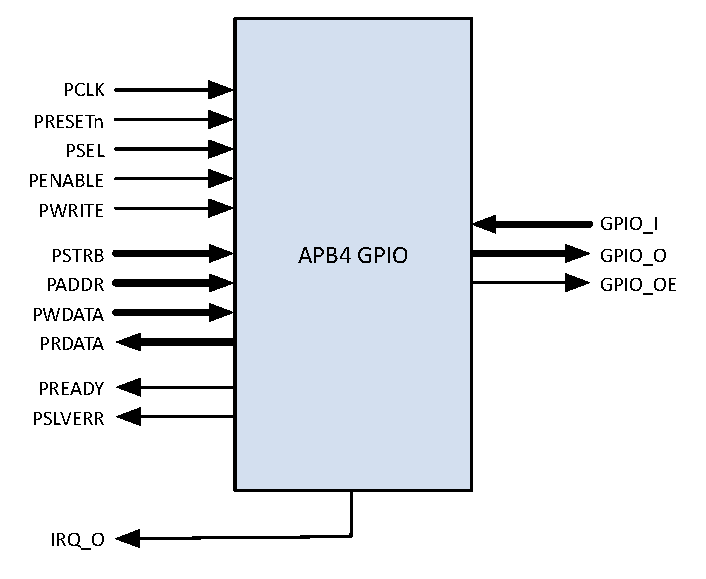
\includegraphics{assets/img/apb4-gpio-sig}
	\caption{APB4 GPIO Signalling}
	\label{fig:apb4-gpio-sig}
\end{figure}

\section{Features}\label{features}

\begin{itemize}
\item
  Compliant with AMBA APB v2.0 Specification
\item
  User-defined number of Bi-directional General Purpose IO
\item
  Automatic synchronisation of General Inputs to Bus Clock
\item
  Each General Output configurable as push-pull or open-drain
\item
  Programmable IRQ generation
\item
  Each General input individually configurable as a level or edge triggered interrupt.
\end{itemize}
